% this file is called up by thesis.tex
% content in this file will be fed into the main document

%: ----------------------- name of chapter  -------------------------
\chapter{Software Design and Analysis} % top level followed by section, subsection


%: ----------------------- paths to graphics ------------------------

% change according to folder and file names
\ifpdf
    \graphicspath{{3/figures/PNG/}{3/figures/PDF/}{3/figures/}}
\else
    \graphicspath{{3/figures/EPS/}{3/figures/}}
\fi

%: ----------------------- contents from here ------------------------
\section{Overview}
In this chapter, the software (Public Transportation Search Web Portal) development life cycle has been discussed.

\section{Software Development Process Model}
A software development process model is simply the process by which an organization 
develops software. (Zeil, 2016). It is broken down into several phases, there are different criteria for each phase \citep{marciniak1994encyclopedia}. The software development model chosen here is the spiral model. This model was chosen due to the exploratory nature of the project.

The spiral model cycles through four quadrants, each representing a particular development phase \cite{boehm_spiral_1988}. The cycle is shown in Figure 3.1.

\begin{figure}[th!]
	\centering
	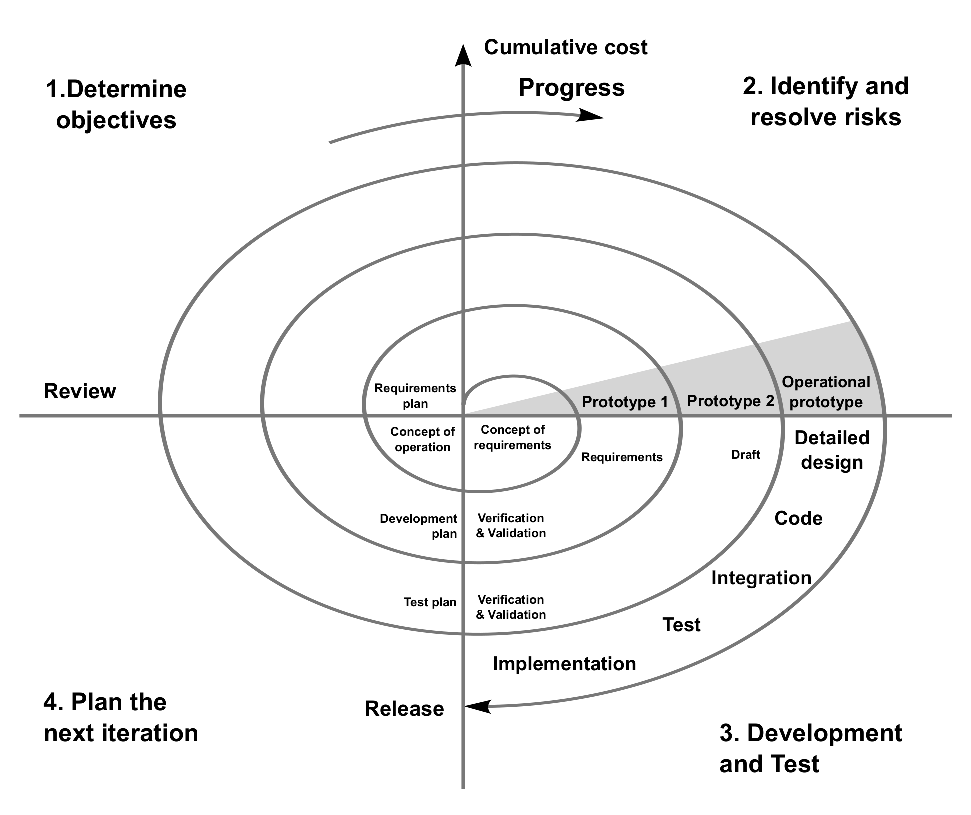
\includegraphics[width=1.0\textwidth]{spiral}
	\caption[The Spiral Model of Software Development]{The Spiral Model of Software Development}
	\label{fig:spiral}
\end{figure}

\subsection{Phases of the Spiral Model}
The phases of the spiral model includes:

\subsubsection{Determine Objectives, Alternatives and Constraints}
During this phase the objectives for the iteration, and it's alternatives and constraints are investigated.

\subsubsection{Evaluate Alternatives, Identify and Resolve Risks}
The risks involved in the iteration of development are examined, and solutions are found. Additionally, this phase also evaluates the alternatives to the chosen strategy.

\subsubsection{Develop and Verify the Next Level Product}
The development of the product takes place in this phase. For each cycle a different methodology may be used during this phase. For instance, the waterfall model can be used for 

\subsubsection{Plan Next Iteration}
During this phase, with all the information gained from the past cycles, the next iteration is planned.

\subsection{Advantages of the Spiral Model}
The advantages of the Spiral Model are as follows:
\begin{itemize}
	\item It enhances risk avoidance;
	\item A different methodology can be selected for each iteration; and 
	\item It can incorporate the Waterfall, Prototype and Incremental methodologies.
\end{itemize}

\section{Feasibility Studies and Analyses}
This section conducts a feasibility study on the project, and analyses  the cost and risk involved.

\subsection{Cost Analysis}
Since this is a software only project we will not concern ourselves with price of hardware.  However, the price of the hardware is directly to the resources used, which were analysed in the feasibility study. Therefore it is concluded hat this system will be relatively inexpensive to run.

\subsection{Risk Analysis}

\subsection{Use Case Diagram}

\subsection{Activity Diagram}

\section{Implementation}
The application is set into operation at the implementation stage. This includes how data is taken by the system, what form of data is taken by the system, where the data is kept, how the data is processed and what form of information is outputted.The first step was to map out collected transport terminals detailed information; including but no limited to:
\begin{itemize}
	\item Name
	\item Location (Town name)
	\item Location (Longitude and Latitude)
	\item Contacts (Phone, Email, Website, Operator)
	\item Operators (STC, GRPTU, VVIP, VIP)
\end{itemize}

in some parts of Ghana. The mapped data was uploaded to OpenStreetMap database. After the mapping of the lorry stations, the mapped data was downloaded and processed in QGIS before being imported into the projects PostgreSQL based database.

\subsection{Mapping Transportation Terminals}
The following steps were taken in the mapping out process:
\begin{itemize}
	\item Go to \textit{www.osm.org} in a modern web browser such as Firefox of Chromium; 
	\item Searched for town or city where lorry station is to be mapped; and 
	\item Area was edited by: 
	\item Marking out specific areas (buildings, routes (roads, walkways) and the stations are either mapped as points or closed ways (polygons);  
	\item Naming  and describing of point, areas or routes. 
\end{itemize}

\textit{Insert image of update / mapped terminals}

\subsection{Data Collection}
The following information were collected from the selected lorry stations. Some of these information was collected by survey and crowdsouring.
\begin{itemize}
	\item Name;
	\item Operator;
	\item Departure time;
	\item Fares; and 
	\item Available destinations.
\end{itemize}

\textit{Insert image of tickets / terminal schedule board}

% ---------------------------------------------------------------------------
%: ----------------------- end of thesis sub-document ------------------------
% ---------------------------------------------------------------------------

